\section{Ciepły start}\label{chapter:results_warm_start}

Pierwszym kryterium badanym w testach wydajnościowych był czas działania funkcji podczas ciepłych startów.
Oznacza to sytuację, gdy funkcja była wywołana w momencie, gdy aktywna była jedna z instancji funkcji.
Powoduje to, że nie jest wymagana inicjalizacja usługi, a kod rozpoczyna działanie bezpośrednio po wywołaniu.
W badaniu każda funkcja została wywołana stukrotnie, a wyniki zostały zagregowane.
Średni czas wykonania w zależności od metody i rozmiaru pamięci został przedstawiony na Rysunku \ref{fig:avg_warm_start}.
Dokładne wartości badanych parametrów (czas średni, mediana, odchylenie standardowe) i różnice względem funkcji bazowej (Java JVM) zostały zaprezentowane w Tabeli \ref{table:warm_start_comparison}.
Dla wszystkich badanych grup wykonano test Shapiro-Wilka, który wykazał, że jedynie dwie z badanych grup wykazywały rozkład normalny (funkcje SnapStart dla pamięci 128 MB).
Ze względu na brak normalności rozkładu pozostałych, przeprowadzono test Kruskal-Wallis, którego wyniki zostały przedstawione w Tabeli \ref{table:kruskal_wallis_test_warm_starts}.
Jego wyniki były zbliżone do zera (oraz poniżej poziomu istotności $\alpha = 0,05$), zatem wykonano test Dunn (którego wyniki zaprezentowano w Tabeli \ref{table:dunn_results_warm_starts}).

\begin{table}[h!]
    \centering
    \caption{Wyniki testu Kruskal-Wallis dla wyników pomiaru czasu działania funkcji podczas ciepłych startów [źródło: opracowanie własne]}
    \begin{tabular}{|c|c|}
    \hline
    \textbf{Wielkość pamięci [MB]} & \textbf{Wartość p} \\
    \hline
    128 & $6.46 \times 10^{-38}$ \\
    \hline
    256 & $1.65 \times 10^{-18}$ \\
    \hline
    512 & $9.37 \times 10^{-43}$ \\
    \hline
    1024 & $3.62 \times 10^{-72}$ \\
    \hline
    2048 & $1.69 \times 10^{-72}$ \\
    \hline
    \end{tabular}
    \label{table:kruskal_wallis_test_warm_starts}
\end{table}

\begin{figure}[h]
    \centering
    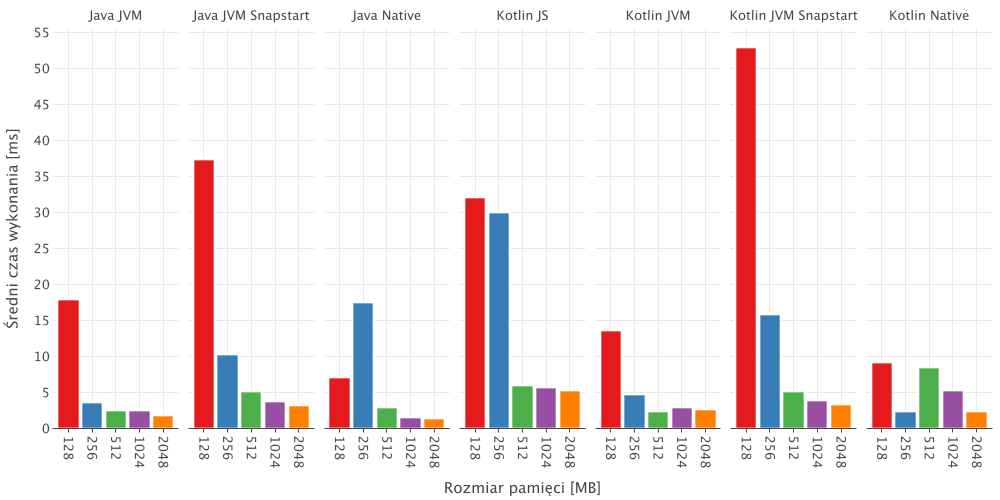
\includegraphics[width=0.95\textwidth]{charts/results/avg-warm-start.png}
    \caption{Średni czas wykonywania funkcji (ciepły start) z użyciem wybranych metod w zależności od rozmiaru pamięci [źródło: opracowanie własne]}
    \label{fig:avg_warm_start}
\end{figure}

Dla każdego z badanych rodzajów funkcji widoczne jest znaczne zróżnicowanie czasu wykonania w zależności od rozmiaru pamięci.
Sama skuteczność metod w poprawie wydajności różni się także ze względu na pamięć funkcji.
Analizy wartości średnich oraz mediany dla pierwszej metody, czyli usługi SnapStart wykazuje, że metoda ta nie przyniosła poprawy czasu wykonania w żadnej z badanych wielkości pamięci.
Istotne różnice wykazał także przeprowadzony test Dunn (którego wyniki zaprezentowano w Tabeli \ref{table:dunn_results_warm_starts}).
W przypadku Javy, wyniki SnapStart są istotnie różne dla pamięci 256 MB, 1024 MB i 2048 MB dla przyjętego poziomu istotności.
Dla pozostałych rozmiarów pamięci (128 MB, 512 MB) wartość p nie była jednak także wysoka i wynosi około 0,08.
W przypadku Kotlina, test Dunn pozwolił odrzucić hipotezę zerową dla wszystkich rozmiarów pamięci oprócz 1024 MB, gdzie wyniki były zbliżone. 

W ramach funkcji opartych o JVM, użycie Kotlina w miejscu Javy nie przyniosło znacznych różnic w wydajności.
Analiza wyników testu Dunn wykazała jedynie znaczną różnicę w przypadku funkcji o pamięci 2048 MB, gdzie Java pozwoliła na istotnie krótszy czas działania.
Wartość średnia oraz mediana jest niższa dla funkcji Kotlin dla pamięci 128 MB i 512 MB.
Różnica nie jest jednak na tyle znacząca, by możliwe było potwierdzenie tego faktu testem Dunn.
Dla pamięci 512 MB, wartość p wynosi jednak około 0,9, zatem metoda ta była najbliższa poprawie wydajności w tym konkretnym scenariuszu. 

Trudnym w ocenie przypadkiem są funkcje oparte o Kotlin/JS.
Według przewidywań, użycie języka intepretowanego powinno zapewnić istotnie dłuższy czas procesowania względem języków kompilowanych (Java i Kotlin).
Kotlin/JS cechuje się bardzo dużą różnicą między wartością średnią i medianą oraz wartością odchylenia standardowego.
Oznacza to bardzo dużą niestabilność wyników.
Dla wszystkich rozmiarów funkcji średni czas działania był wyższy niż dla analogicznych funkcji Java JVM i Kotlin JVM.
Mediany były jednak niższe dla rozmiarów 128 MB i 512 MB.
Test Dunn nie pozwolił na odrzucenie hipotezy zerowej pomiędzy Kotlin/JS oraz Java JVM i Kotlin JVM dla pamięci 128 MB, 512 MB i 10224 MB.
Dla pamięci 256 MB i 2048 MB możliwe jest stwierdzenie o istotnie negatywnym wpływie Kotlin/JS na czas działania funkcji.
Dla pozostałych pamięci średni czas działania funkcji wykazuje także negatywny wpływ, jednak niemożliwie jest statystyczne potwierdzenie tego faktu.
Może to wynikać z niestabilności działania Kotlin/JS, na co wpływ może mieć natura języka JavaScript.

Zastosowanie obrazów natywnych GraalVM pozwala na zmniejszenie czasu w niektórych rozmiarach pamięci: 128 MB, 1024 MB oraz 2048 MB.
Dla tych rozmiarów wartości średnie oraz mediany są niższe niż dla analogicznej funkcji działającej w JVM.
Zostało to także potwierdzone testem Dunn.
Dla pamięci 256 MB i 512 MB, wartości średnie są wyższe dla GraalVM, jednak mediany znacznie niższe.
Test Dunn pozwolił odrzucić hipotezę zerową w przypadku pamięci 512 MB.
Nie jest jednak możliwe stwierdzenie poprawy wydajności dla tych wielkości pamięci, co może wynikać z dużej niestabilności wyników GraalVM.
Ważnym faktem jest również wysoka wartość odchylenia standardowego, która jest wyższa dla GraalVM w każdej z badanych wielkości pamięci.
Może to wskazywać na niestabilność obrazów natywnych GraalVM.

Skuteczność Kotlin/Native zależy znacznie od wielkości pamięci.
Dla dużych rozmiarów (512-2048 MB), metoda ta wpłynęła negatywnie na czas działania.
Wartości średnie i mediany są znacznie wyższe dla tych pamięci, a wyniki testu Dunn pozwalają na stwierdzenie o istotnych różnicach względem funkcji Java JVM. 
Kotlin/Native wpłynął także na czas procesowania w porównaniu z funkcjami Kotlin JVM dla rozmiarów 512 MB i 1024 MB.
Dla największej pamięci 2048 MB, czas działania Kotlin/Native jest jednak zbliżony do Kotlin JVM (test Dunn wykazał wartość p równą 1, zatem różnice nie są znaczne).
W przypadku pamięci małych (128 MB, 256 MB), Kotlin/Native pozwolił na uzyskanie niższych średni czasów wykonania oraz ich median.
Test Dunn nie wskazał jednak na różnicę istotną statystycznie.
Kotlin/Native cechuje się jednak niższym odchyleniem standardowym niż druga metoda oparta o kompilację natywną, czyli GraalVM.
Wartości te są zbliżone dla pamięci 512 MB i 1024 MB, jednak przy dużej różnicy średnich czasów na niekorzyść Kotlin/Native.
Sam Kotlin/Native może jednak także cechować się pewną niestabilnością.
Istotna jest różnica wydajności między pamięciami 128 MB i 256 MB oraz 256 MB i 512 MB.
Dla pierwszej pary czas działania znacznie zmalał wraz z wzrostem pamięci, dla drugiej sytuacja była odwrotna.

\newpage

\begin{table}[!h]
\centering
\caption{Porównanie średnich, median oraz odchyleń standardowych czasów działania funkcji podczas ciepłego startu względem funkcji bazowej (Java JVM) [źródło: opracowanie własne]}
\small
\begin{tabular}{|>{\centering\arraybackslash}m{1.5cm}|l|p{1.5cm}|p{1.5cm}|p{1.5cm}|p{1.5cm}|p{1.5cm}|}
\toprule
Rozmiar pamięci [MB] & Metoda & Średnia [ms] & Zmiana średniej & Mediana [ms] & Zmiana mediany & Odch. stand. \\
\midrule
\multirow{7}{*}{128} & Java JVM & 17.89 & \mbox{0\%} & 14.55 & \mbox{0\%} & 14.02 \\
 & Java GraalVM & 7.09 & \mbox{-60\%} & 1.13 & \mbox{-92\%} & 29.43 \\
 & Java JVM + SnapStart & 37.36 & \mbox{+109\%} & 35.86 & \mbox{+146\%} & 18.88 \\
 & Kotlin JVM & 13.56 & \mbox{-24\%} & 10.32 & \mbox{-29\%} & 19.70 \\
 & Kotlin JVM + SnapStart & 52.92 & \mbox{+196\%} & 44.69 & \mbox{+207\%} & 28.23 \\
 & Kotlin/JS & 32.15 & \mbox{+80\%} & 2.56 & \mbox{-82\%} & 63.63 \\
 & Kotlin/Native & 9.19 & \mbox{-49\%} & 7.08 & \mbox{-51\%} & 7.90 \\
\midrule
\multirow{7}{*}{256} & Java JVM & 3.66 & \mbox{0\%} & 2.16 & \mbox{0\%} & 4.59 \\
 & Java GraalVM & 17.48 & \mbox{+378\%} & 1.25 & \mbox{-42\%} & 24.41 \\
 & Java JVM + SnapStart & 10.31 & \mbox{+182\%} & 11.95 & \mbox{+453\%} & 7.45 \\
 & Kotlin JVM & 4.70 & \mbox{+29\%} & 2.13 & \mbox{-1\%} & 5.80 \\
 & Kotlin JVM + SnapStart & 15.87 & \mbox{+334\%} & 13.41 & \mbox{+521\%} & 12.12 \\
 & Kotlin/JS & 29.98 & \mbox{+720\%} & 10.24 & \mbox{+374\%} & 43.71 \\
 & Kotlin/Native & 2.37 & \mbox{-35\%} & 2.06 & \mbox{-5\%} & 1.70 \\
\midrule
\multirow{7}{*}{512} & Java JVM & 2.56 & \mbox{0\%} & 2.37 & \mbox{0\%} & 0.62 \\
 & Java GraalVM & 2.87 & \mbox{+12\%} & 1.30 & \mbox{-45\%} & 6.34 \\
 & Java JVM + SnapStart & 5.15 & \mbox{+101\%} & 2.86 & \mbox{+21\%} & 4.88 \\
 & Kotlin JVM & 2.41 & \mbox{-6\%} & 2.03 & \mbox{-14\%} & 1.24 \\
 & Kotlin JVM + SnapStart & 5.13 & \mbox{+101\%} & 2.94 & \mbox{+24\%} & 5.26 \\
 & Kotlin/JS & 5.94 & \mbox{+132\%} & 1.97 & \mbox{-17\%} & 11.96 \\
 & Kotlin/Native & 8.45 & \mbox{+231\%} & 6.80 & \mbox{+187\%} & 6.35 \\
\midrule
\multirow{7}{*}{1024} & Java JVM & 2.48 & \mbox{0\%} & 2.42 & \mbox{0\%} & 0.27 \\
 & Java GraalVM & 1.48 & \mbox{-40\%} & 1.01 & \mbox{-58\%} & 2.44 \\
 & Java JVM + SnapStart & 3.74 & \mbox{+51\%} & 2.92 & \mbox{+21\%} & 2.30 \\
 & Kotlin JVM & 2.89 & \mbox{+17\%} & 2.75 & \mbox{+14\%} & 0.95 \\
 & Kotlin JVM + SnapStart & 3.89 & \mbox{+57\%} & 3.09 & \mbox{+28\%} & 1.80 \\
 & Kotlin/JS & 5.66 & \mbox{+129\%} & 3.04 & \mbox{+26\%} & 6.65 \\
 & Kotlin/Native & 5.31 & \mbox{+114\%} & 6.57 & \mbox{+171\%} & 2.13 \\
\midrule
\multirow{7}{*}{2048} & Java JVM & 1.81 & \mbox{0\%} & 1.44 & \mbox{0\%} & 0.70 \\
 & Java GraalVM & 1.40 & \mbox{-23\%} & 1.07 & \mbox{-26\%} & 1.75 \\
 & Java JVM + SnapStart & 3.26 & \mbox{+80\%} & 2.80 & \mbox{+94\%} & 1.01 \\
 & Kotlin JVM & 2.62 & \mbox{+44\%} & 2.12 & \mbox{+47\%} & 1.19 \\
 & Kotlin JVM + SnapStart & 3.40 & \mbox{+88\%} & 2.88 & \mbox{+100\%} & 1.63 \\
 & Kotlin/JS & 5.26 & \mbox{+190\%} & 4.02 & \mbox{+179\%} & 3.76 \\
 & Kotlin/Native & 2.36 & \mbox{+30\%} & 2.24 & \mbox{+56\%} & 0.38 \\
\bottomrule
\end{tabular}
\label{table:warm_start_comparison}
\end{table}

% % --- Row 1: 256 MB and 1024 MB charts ---
% \begin{figure}[h]
%     \centering % Center the minipages on the line
%     \begin{minipage}[t]{0.48\textwidth} % [t] for top alignment
%         \centering % Center content within this minipage
%         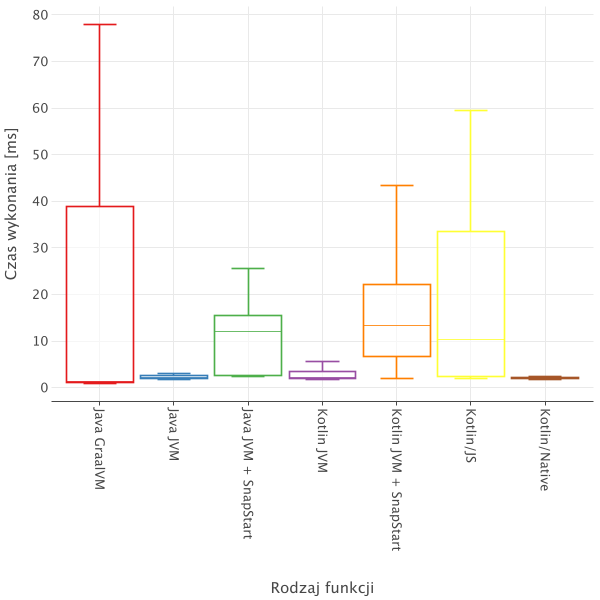
\includegraphics[width=\linewidth]{charts/results/warm-start-boxplot-256.png}
%         \captionof{figure}{Czas wykonania funkcji (ciepły start, 256 MB) [źródło: opracowanie własne]}
%         \label{fig:warm_start_256} % Unique label for this figure
%     \end{minipage}% <--- % is important
%     \hfill % Space between minipages
%     \begin{minipage}[t]{0.48\textwidth}
%         \centering
%         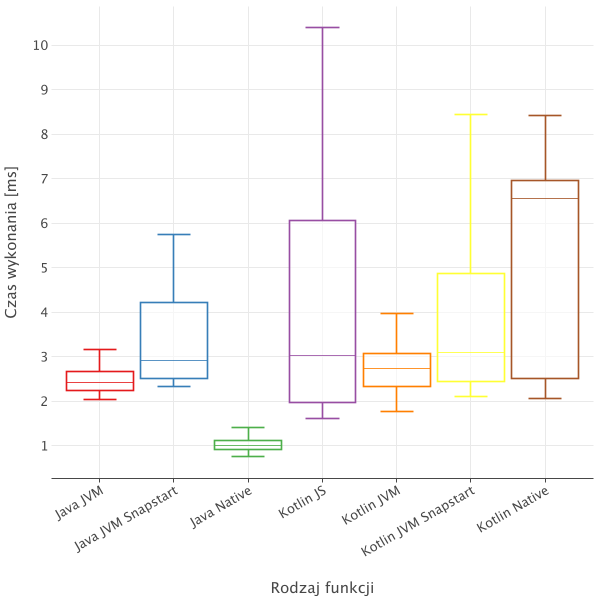
\includegraphics[width=\linewidth]{charts/results/warm-start-boxplot-1024.png}
%         \captionof{figure}{Czas wykonania funkcji (ciepły start, 1024 MB) [źródło: opracowanie własne]}
%         \label{fig:warm_start_1024} % Unique label
%     \end{minipage}
%     % No overall \caption for this outer figure environment, as it's just for layout.
% \end{figure}

\begin{table}[!h]
    \caption{Porównanie czasów działania funkcji podczas ciepłych startów poprzez wartość p testu Dunn (\textbf{istotne różnice pogrubione}) [źródło: opracowanie własne]}
    \centering
    \footnotesize
    \begin{tabular}{|p{3cm}|>{\raggedright\arraybackslash}p{3cm}|>{\raggedright\arraybackslash}p{1.5cm}|>{\raggedright\arraybackslash}p{1.5cm}|>{\raggedright\arraybackslash}p{1.5cm}|>{\raggedright\arraybackslash}p{1.5cm}|>{\raggedright\arraybackslash}p{1.5cm}|}
    \hline
    \multirow{2}{*}{\textbf{Pierwsza funkcja}} & \multirow{2}{*}{\textbf{Druga funkcja}} & \multicolumn{5}{c|}{\textbf{Wielkość pamięci [MB]}} \\
    \cline{3-7}
    & & \textbf{128} & \textbf{256} & \textbf{512} & \textbf{1024} & \textbf{2048} \\
    \hline
    \multirow{6}{*}{Java GraalVM} & Java JVM & $\bm{5.44 \times 10^{-16}}$ & 0.7368 & $\bm{5.51 \times 10^{-11}}$ & $\bm{1.93 \times 10^{-9}}$ & $\bm{2.08 \times 10^{-16}}$ \\ 
    \cline{2-7}
    & Java JVM + SnapStart & $\bm{1.29 \times 10^{-25}}$ & $\bm{4.78 \times 10^{-8}}$ & $\bm{1.48 \times 10^{-19}}$ & $\bm{2.65 \times 10^{-21}}$ & $\bm{2.52 \times 10^{-34}}$ \\
    \cline{2-7}
    & Kotlin JVM & $\bm{9.37 \times 10^{-10}}$ & 0.6159 & $\bm{9.01 \times 10^{-5}}$ & $\bm{4.54 \times 10^{-32}}$ & $\bm{5.90 \times 10^{-19}}$ \\
    \cline{2-7}
    & Kotlin JVM + SnapStart & $\bm{4.27 \times 10^{-32}}$ & $\bm{5.80 \times 10^{-10}}$ & $\bm{2.98 \times 10^{-18}}$ & $\bm{9.73 \times 10^{-21}}$ & $\bm{8.19 \times 10^{-33}}$ \\
    \cline{2-7}
    & Kotlin/JS & $\bm{6.55 \times 10^{-15}}$ & $\bm{3.89 \times 10^{-10}}$ & $\bm{3.05 \times 10^{-9}}$ & $\bm{3.32 \times 10^{-20}}$ & $\bm{8.88 \times 10^{-39}}$ \\
    \cline{2-7}
    & Kotlin/Native & $\bm{9.37 \times 10^{-10}}$ & 1.0000 & $\bm{3.86 \times 10^{-34}}$ & $\bm{1.11 \times 10^{-66}}$ & $\bm{1.37 \times 10^{-19}}$ \\
    \hline
    \multirow{5}{*}{Java JVM} & Java JVM + SnapStart & 0.0740 & \textbf{0.0042} & 0.0835 & \textbf{0.0359} & $\bm{1.89 \times 10^{-10}}$ \\
    \cline{2-7}
    & Kotlin JVM & 0.3281 & 1.0000 & 0.0893 & 0.4362 & \textbf{0.0153} \\
    \cline{2-7}
    & Kotlin JVM + SnapStart & \textbf{0.0011} & $\bm{5.69 \times 10^{-4}}$ & 0.1263 & \textbf{0.0329} & $\bm{2.38 \times 10^{-9}}$ \\
    \cline{2-7}
    & Kotlin/JS & 0.1164 & $\bm{6.92 \times 10^{-4}}$ & 0.1195 & 0.1252 & $\bm{8.36 \times 10^{-12}}$ \\
    \cline{2-7}
    & Kotlin/Native & 0.3281 & 1.0000 & $\bm{5.70 \times 10^{-4}}$ & $\bm{5.29 \times 10^{-8}}$ & \textbf{0.0104} \\
    \hline
    \multirow{4}{\linewidth}{Java JVM + SnapStart} & Kotlin JVM & $\bm{9.08 \times 10^{-5}}$ & \textbf{0.0057} & $\bm{8.12 \times 10^{-6}}$ & 0.4362 & \textbf{0.0153} \\
    \cline{2-7}
    & Kotlin JVM + SnapStart & 0.9682 & 1.0000 & 1.0000 & 1.0000 & 1.0000 \\
    \cline{2-7}
    & Kotlin/JS & $\bm{7.12 \times 10^{-7}}$ & 1.0000 & $\bm{1.09 \times 10^{-6}}$ & 1.0000 & 1.0000 \\
    \cline{2-7}
    & Kotlin/Native & $\bm{9.08 \times 10^{-5}}$ & $\bm{1.06 \times 10^{-4}}$ & 1.0000 & 0.3242 & \textbf{0.0180} \\
    \hline
    \multirow{3}{*}{Kotlin JVM} & Kotlin JVM + SnapStart & $\bm{1.59 \times 10^{-7}}$ & $\bm{7.84 \times 10^{-4}}$ & $\bm{3.48 \times 10^{-5}}$ & 0.4362 & \textbf{0.0349} \\
    \cline{2-7}
    & Kotlin/JS & 1.0000 & $\bm{9.48 \times 10^{-4}}$ & 1.0000 & 0.8655 & \textbf{0.0106} \\
    \cline{2-7}
    & Kotlin/Native & 1.0000 & 1.0000 & $\bm{5.51 \times 10^{-11}}$ & $\bm{5.91 \times 10^{-8}}$ & 1.0000 \\
    \hline
    \multirow{2}{\linewidth}{Kotlin JVM + SnapStart} & Kotlin/JS & $\bm{5.86 \times 10^{-11}}$ & 1.0000 & $\bm{8.12 \times 10^{-6}}$ & 1.0000 & 1.0000 \\
    \cline{2-7}
    & Kotlin/Native & $\bm{1.59 \times 10^{-7}}$ & $\bm{7.13 \times 10^{-6}}$ & 0.8982 & 0.4362 & \textbf{0.0427} \\
    \hline
    Kotlin/JS & Kotlin/Native & 1.0000 & $\bm{8.07 \times 10^{-6}}$ & $\bm{2.04 \times 10^{-17}}$ & \textbf{0.0466} & \textbf{0.0153} \\
    \hline
    \end{tabular}
    \label{table:dunn_results_warm_starts}
\end{table}

\newpage